\documentclass{article}
\usepackage[margin=1in]{geometry}
\usepackage{amsmath}
\usepackage{amsfonts}
\usepackage{graphicx}
\usepackage{xcolor}
\usepackage{ulem}
\usepackage{hyperref}
% Calligraphic fonts
\newcommand{\calA}{{\cal A}}
\newcommand{\calB}{{\cal B}}
\newcommand{\calC}{{\cal C}}
\newcommand{\calD}{{\cal D}}
\newcommand{\calE}{{\cal E}}
\newcommand{\calF}{{\cal F}}
\newcommand{\calG}{{\cal G}}
\newcommand{\calH}{{\cal H}}
\newcommand{\calI}{{\cal I}}
\newcommand{\calJ}{{\cal J}}
\newcommand{\calK}{{\cal K}}
\newcommand{\calL}{{\cal L}}
\newcommand{\calM}{{\cal M}}
\newcommand{\calN}{{\cal N}}
\newcommand{\calO}{{\cal O}}
\newcommand{\calP}{{\cal P}}
\newcommand{\calQ}{{\cal Q}}
\newcommand{\calR}{{\cal R}}
\newcommand{\calS}{{\cal S}}
\newcommand{\calT}{{\cal T}}
\newcommand{\calU}{{\cal U}}
\newcommand{\calV}{{\cal V}}
\newcommand{\calW}{{\cal W}}
\newcommand{\calX}{{\cal X}}
\newcommand{\calY}{{\cal Y}}
\newcommand{\calZ}{{\cal Z}}

% Sets:
\newcommand{\setA}{\textsf{A}}
\newcommand{\setB}{\textsf{B}}
\newcommand{\setC}{\textsf{C}}
\newcommand{\setD}{\textsf{D}}
\newcommand{\setE}{\textsf{E}}
\newcommand{\setF}{\textsf{F}}
\newcommand{\setG}{\textsf{G}}
\newcommand{\setH}{\textsf{H}}
\newcommand{\setI}{\textsf{I}}
\newcommand{\setJ}{\textsf{J}}
\newcommand{\setK}{\textsf{K}}
\newcommand{\setL}{\textsf{L}}
\newcommand{\setM}{\textsf{M}}
\newcommand{\setN}{\textsf{N}}
\newcommand{\setO}{\textsf{O}}
\newcommand{\setP}{\textsf{P}}
\newcommand{\setQ}{\textsf{Q}}
\newcommand{\setR}{\textsf{R}}
\newcommand{\setS}{\textsf{S}}
\newcommand{\setT}{\textsf{T}}
\newcommand{\setU}{\textsf{U}}
\newcommand{\setV}{\textsf{V}}
\newcommand{\setW}{\textsf{W}}
\newcommand{\setX}{\textsf{X}}
\newcommand{\setY}{\textsf{Y}}
\newcommand{\setZ}{\textsf{Z}}

% Vectors
\newcommand{\bfa}{\mathbf{a}}
\newcommand{\bfb}{\mathbf{b}}
\newcommand{\bfc}{\mathbf{c}}
\newcommand{\bfd}{\mathbf{d}}
\newcommand{\bfe}{\mathbf{e}}
\newcommand{\bff}{\mathbf{f}}
\newcommand{\bfg}{\mathbf{g}}
\newcommand{\bfh}{\mathbf{h}}
\newcommand{\bfi}{\mathbf{i}}
\newcommand{\bfj}{\mathbf{j}}
\newcommand{\bfk}{\mathbf{k}}
\newcommand{\bfl}{\mathbf{l}}
\newcommand{\bfm}{\mathbf{m}}
\newcommand{\bfn}{\mathbf{n}}
\newcommand{\bfo}{\mathbf{o}}
\newcommand{\bfp}{\mathbf{p}}
\newcommand{\bfq}{\mathbf{q}}
\newcommand{\bfr}{\mathbf{r}}
\newcommand{\bfs}{\mathbf{s}}
\newcommand{\bft}{\mathbf{t}}
\newcommand{\bfu}{\mathbf{u}}
\newcommand{\bfv}{\mathbf{v}}
\newcommand{\bfw}{\mathbf{w}}
\newcommand{\bfx}{\mathbf{x}}
\newcommand{\bfy}{\mathbf{y}}
\newcommand{\bfz}{\mathbf{z}}


\newcommand{\bfalpha}{\boldsymbol{\alpha}}
\newcommand{\bfbeta}{\boldsymbol{\beta}}
\newcommand{\bfgamma}{\boldsymbol{\gamma}}
\newcommand{\bfdelta}{\boldsymbol{\delta}}
\newcommand{\bfepsilon}{\boldsymbol{\epsilon}}
\newcommand{\bfzeta}{\boldsymbol{\zeta}}
\newcommand{\bfeta}{\boldsymbol{\eta}}
\newcommand{\bftheta}{\boldsymbol{\theta}}
\newcommand{\bfiota}{\boldsymbol{\iota}}
\newcommand{\bfkappa}{\boldsymbol{\kappa}}
\newcommand{\bflambda}{\boldsymbol{\lambda}}
\newcommand{\bfmu}{\boldsymbol{\mu}}
\newcommand{\bfnu}{\boldsymbol{\nu}}
\newcommand{\bfomicron}{\boldsymbol{\omicron}}
\newcommand{\bfpi}{\boldsymbol{\pi}}
\newcommand{\bfrho}{\boldsymbol{\rho}}
\newcommand{\bfsigma}{\boldsymbol{\sigma}}
\newcommand{\bftau}{\boldsymbol{\tau}}
\newcommand{\bfupsilon}{\boldsymbol{\upsilon}}
\newcommand{\bfphi}{\boldsymbol{\phi}}
\newcommand{\bfchi}{\boldsymbol{\chi}}
\newcommand{\bfpsi}{\boldsymbol{\psi}}
\newcommand{\bfomega}{\boldsymbol{\omega}}
\newcommand{\bfxi}{\boldsymbol{\xi}}
\newcommand{\bfell}{\boldsymbol{\ell}}

% Matrices
\newcommand{\bfA}{\mathbf{A}}
\newcommand{\bfB}{\mathbf{B}}
\newcommand{\bfC}{\mathbf{C}}
\newcommand{\bfD}{\mathbf{D}}
\newcommand{\bfE}{\mathbf{E}}
\newcommand{\bfF}{\mathbf{F}}
\newcommand{\bfG}{\mathbf{G}}
\newcommand{\bfH}{\mathbf{H}}
\newcommand{\bfI}{\mathbf{I}}
\newcommand{\bfJ}{\mathbf{J}}
\newcommand{\bfK}{\mathbf{K}}
\newcommand{\bfL}{\mathbf{L}}
\newcommand{\bfM}{\mathbf{M}}
\newcommand{\bfN}{\mathbf{N}}
\newcommand{\bfO}{\mathbf{O}}
\newcommand{\bfP}{\mathbf{P}}
\newcommand{\bfQ}{\mathbf{Q}}
\newcommand{\bfR}{\mathbf{R}}
\newcommand{\bfS}{\mathbf{S}}
\newcommand{\bfT}{\mathbf{T}}
\newcommand{\bfU}{\mathbf{U}}
\newcommand{\bfV}{\mathbf{V}}
\newcommand{\bfW}{\mathbf{W}}
\newcommand{\bfX}{\mathbf{X}}
\newcommand{\bfY}{\mathbf{Y}}
\newcommand{\bfZ}{\mathbf{Z}}


\newcommand{\bfGamma}{\boldsymbol{\Gamma}}
\newcommand{\bfDelta}{\boldsymbol{\Delta}}
\newcommand{\bfTheta}{\boldsymbol{\Theta}}
\newcommand{\bfLambda}{\boldsymbol{\Lambda}}
\newcommand{\bfPi}{\boldsymbol{\Pi}}
\newcommand{\bfSigma}{\boldsymbol{\Sigma}}
\newcommand{\bfUpsilon}{\boldsymbol{\Upsilon}}
\newcommand{\bfPhi}{\boldsymbol{\Phi}}
\newcommand{\bfPsi}{\boldsymbol{\Psi}}
\newcommand{\bfOmega}{\boldsymbol{\Omega}}


% Blackboard Bold:
\newcommand{\bbA}{\mathbb{A}}
\newcommand{\bbB}{\mathbb{B}}
\newcommand{\bbC}{\mathbb{C}}
\newcommand{\bbD}{\mathbb{D}}
\newcommand{\bbE}{\mathbb{E}}
\newcommand{\bbF}{\mathbb{F}}
\newcommand{\bbG}{\mathbb{G}}
\newcommand{\bbH}{\mathbb{H}}
\newcommand{\bbI}{\mathbb{I}}
\newcommand{\bbJ}{\mathbb{J}}
\newcommand{\bbK}{\mathbb{K}}
\newcommand{\bbL}{\mathbb{L}}
\newcommand{\bbM}{\mathbb{M}}
\newcommand{\bbN}{\mathbb{N}}
\newcommand{\bbO}{\mathbb{O}}
\newcommand{\bbP}{\mathbb{P}}
\newcommand{\bbQ}{\mathbb{Q}}
\newcommand{\bbR}{\mathbb{R}}
\newcommand{\bbS}{\mathbb{S}}
\newcommand{\bbT}{\mathbb{T}}
\newcommand{\bbU}{\mathbb{U}}
\newcommand{\bbV}{\mathbb{V}}
\newcommand{\bbW}{\mathbb{W}}
\newcommand{\bbX}{\mathbb{X}}
\newcommand{\bbY}{\mathbb{Y}}
\newcommand{\bbZ}{\mathbb{Z}}





\title{ECE 417 Midterm 2 2022 practice problem set}
\date{March 30th, 2021}
\author{Instructor: Vikas Dhiman}

\newtheorem{prob}{Problem}
\newif\ifsol
\solfalse

\begin{document}
\maketitle
%$ \hat{\mathbf{w}} = \hat{\mathbf{k}} \times \frac{\mathbf{v}}{\|\mathbf{v}\|} $
%$ \|\hat{\mathbf{w}}\| = \|\hat{\mathbf{k}}\| \|\frac{\mathbf{v}}{\|\mathbf{v}\|}\| \sin(\phi) $. 

\begin{tabular}{p{0.5\linewidth}p{0.5\linewidth}}
  (1) Student name:& Student email: \\
\end{tabular}

\subsubsection*{About the exam}
\begin{enumerate}
  \item There are total 5 problems. You must attempt all 5. 
  \item Maximum marks: 50 (70 with bonus marks).
  \item Maximum time allotted:  50 min
  \item Calculators are allowed.
  \item One US Letter size or A4 size cheat sheet (both-sides) is allowed.
\end{enumerate}

\newcommand{\ubfu}{\underline{\bfu}}
\newcommand{\ubfX}{\underline{\bfX}}
\newpage
\begin{prob}
  Given a set of $n \ge 6$ points $\ubfX_i \in \bbP^3$ for all $i \in \{1,
  \dots, n\}$ in 3D projective space, and a set
  of corresponding points $\ubfu_i \in \bbP^2$ in an image, find the 3D to 2D projective
  $P \in \bbR^{3 \times 4}$ matrix
  that converts $\bfX_i$ to $\ubfu_i  =  \lambda_i P\ubfX_i$. In other words,
  convert $\ubfu_i \times P\ubfX_i = 0$ into a familiar form $A\bfy = \bfb$ or
  $A\bfy = \mathbf{0}$ so that we can solve for $P$. For notation purposes, you can
  denote $\ubfu_i = [x_i, y_i, w_i]^\top$ and $P = \begin{bmatrix}
    \bfp_1^\top \\ \bfp_2^\top \\ \bfp_3^\top \end{bmatrix}$ where $\bfp_1,
  \bfp_2, \bfp_3 \in \bbR^4$ are the rows of $P$ represented as 4-D column vectors.
  (Practical motivation:
    We did camera calibration in lab using a single checker board. It is much
    easier to compute camera calibration using two mutually perpendicular checker
    boards so that all points do not lie on a single plane (hence linearly
    independent). One can make a coordinate system attached to the double checker
    and compute the 3D coordinates of each corner point in that system. Let
    $\ubfX_i \in \bbP^3$ be such points in 3D on the checker-board. Let $\ubfu_i
    \in \bbP^2$ be a point detected in the image so that we have one-to-one
    correspondence between $\ubfX_i$ and $\ubfu_i$. Finding the projection matrix
    $P \in \bbR^{3 \times 4}$ then reduces to the above problem. We will cover
    the breakdown of $P$ matrix into $P = K[R, t]$ in class.
  ) \\
  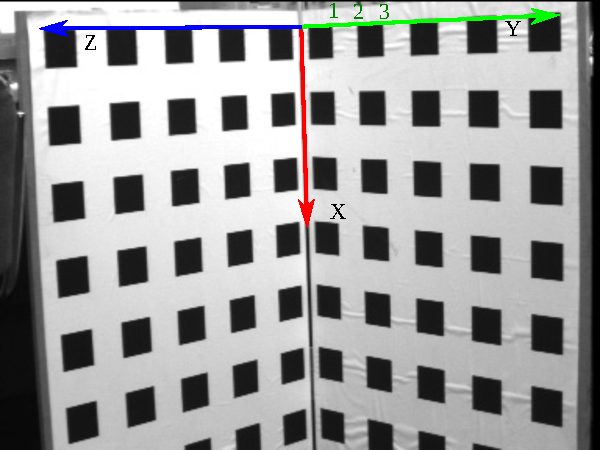
\includegraphics[width=0.5\linewidth]{media/camera-calibration-rig.png.pdf}
\end{prob}
\newpage
\paragraph*{Solution}
Watch lecture \url{https://drive.google.com/file/d/1cY02DTagpckbYl5gS0PYBu569vlZUNN6/view?usp=sharing}
\begin{enumerate}
\item Write cross product as a matrix operation
  \[ [\ubfu_i]_{\times}= \begin{bmatrix}
      0 & -w_i & y_i \\
      w_i & 0 & -x_i \\
      -y_i & x_i & 0
    \end{bmatrix}\]
  \item Write $P \ubfX_i$ in terms of row vectors.
    \[ P \ubfX_i = \begin{bmatrix}
        \bfp_1^\top
        \\
        \bfp_2^\top
        \\
        \bfp_3^\top
      \end{bmatrix}\ubfX_i =  \begin{bmatrix}
        \bfp_1^\top\ubfX_i
        \\
        \bfp_2^\top\ubfX_i
        \\
        \bfp_3^\top\ubfX_i
      \end{bmatrix}\]
    \item Note that all the three terms like $\bfp_1^\top \ubfX_i$ are scalars
      hence they are symmetric. Hence $\bfp_1^\top \ubfX_i = \ubfX_i^\top \bfp_1$ .
      \[ P \ubfX_i = \begin{bmatrix}
          \ubfX_i^\top\bfp_1
                 \\
          \ubfX_i^\top \bfp_2
                 \\
          \ubfX_i^\top\bfp_3
        \end{bmatrix}\]
    \item Substitute these values in the original equation $\ubfu_i \times
      P\ubfX_i = \mathbf{0}_{3\times 1}$.
      \[
        \begin{bmatrix}
          0 & -w_i & y_i \\
          w_i & 0 & -x_i \\
          -y_i & x_i & 0
        \end{bmatrix}
        \begin{bmatrix}
          \ubfX_i^\top\bfp_1
          \\
          \ubfX_i^\top \bfp_2
          \\
          \ubfX_i^\top\bfp_3
        \end{bmatrix} = \mathbf{0}_{3 \times 1}
        \]
      \item Matrix multiply
        \[
          \begin{bmatrix}
            0 -w_i \ubfX_i^\top\bfp_2 + y_i \ubfX_i^\top\bfp_3 \\
            w_i \ubfX_i^\top\bfp_1 + 0  -x_i \ubfX_i^\top\bfp_3 \\
            -y_i \ubfX_i^\top\bfp_1 + x_i \ubfX_i^\top\bfp_2 + 0
          \end{bmatrix} = \mathbf{0}_{3 \times 1}
          \]
        \item Write the unknowns as a single vector, and the knowns as a matrix
          multiplication with the unknowns
          \[
            \begin{bmatrix}
              \mathbf{0}^\top & -w_i \ubfX_i^\top & y_i \ubfX_i^\top \\
              w_i \ubfX_i^\top & \mathbf{0}^\top  & -x_i \ubfX_i^\top \\
              -y_i \ubfX_i^\top & x_i \ubfX_i^\top & \mathbf{0}^\top
              \end{bmatrix}_{3 \times 12}
              \begin{bmatrix}
                \bfp_1 \\
                \bfp_2 \\
                \bfp_3
                \end{bmatrix}_{12 \times 1}
                = \mathbf{0}_{3 \times 1}
            \]
     \item Pick only two of the equations as only two are linearly independent.
       \[
         \begin{bmatrix}
           \mathbf{0}^\top & -w_i \ubfX_i^\top & y_i \ubfX_i^\top \\
           w_i \ubfX_i^\top & \mathbf{0}^\top  & -x_i \ubfX_i^\top
         \end{bmatrix}_{2 \times 12}
         \begin{bmatrix}
           \bfp_1 \\
           \bfp_2 \\
           \bfp_3
         \end{bmatrix}_{12 \times 1}
         = \mathbf{0}_{2 \times 1}
       \]
     \item Collect all the equations from $n$ pairs of corresponding points
       $\ubfu_1, \dots, \ubfu_n$ and $\ubfX_1, \dots, \ubfX_n$.
       \[
         \begin{bmatrix}
           \mathbf{0}^\top & -w_1 \ubfX_1^\top & y_1 \ubfX_1^\top \\
           w_1 \ubfX_1^\top & \mathbf{0}^\top  & -x_1 \ubfX_1^\top \\
           \vdots & \vdots & \vdots\\
           \mathbf{0}^\top & -w_n \ubfX_n^\top & y_n \ubfX_n^\top \\
           w_n \ubfX_n^\top & \mathbf{0}^\top  & -x_n \ubfX_n^\top \\
         \end{bmatrix}_{2n \times 12}
         \begin{bmatrix}
           \bfp_1 \\
           \bfp_2 \\
           \bfp_3
         \end{bmatrix}_{12 \times 1}
         = \mathbf{0}_{2n \times 1}
       \]
   \item $P$ matrix has rank $\text{rank}(P) = 11$ because it has 12 elements
     and equivalence upto a scale factor. So the solution of the above equation
     can be computed from SVD by choosing the right singular vector corresponding
     to the smallest singular value.
     \[
      A = \begin{bmatrix}
        \mathbf{0}^\top & -w_1 \ubfX_1^\top & y_1 \ubfX_1^\top \\
        w_1 \ubfX_1^\top & \mathbf{0}^\top  & -x_1 \ubfX_1^\top \\
        \vdots & \vdots & \vdots\\
        \mathbf{0}^\top & -w_n \ubfX_n^\top & y_n \ubfX_n^\top \\
        w_n \ubfX_n^\top & \mathbf{0}^\top  & -x_n \ubfX_n^\top \\
       \end{bmatrix} = U\Sigma V^T
     \]
     Let $V = [\bfv_1, \dots, \bfv_n]$, then
     \[
       \begin{bmatrix}
         \bfp_1 \\
         \bfp_2 \\
         \bfp_3
         \end{bmatrix} = \bfv_n
       \]

       Now we can write the $P$ matrix as
       \[
         P = \begin{bmatrix}
           \bfp_1^\top \\
           \bfp_2^\top \\
           \bfp_3^\top
         \end{bmatrix}
         \]
\end{enumerate}
\newpage

\begin{prob}
  In figure~\ref{fig:line-plane-triangulation} find the 3D representation of the
  lane the World coordinate frame, in terms of $h$ (the height of the camera),
  image-representation of the line $\bfl$ (provided in figure), camera matrix
  $K$ (provided in figure). Assume the lane to be a straight line.
  The Camera is mounted directly on top of the
  world frame, both of which are aligned to the gravity vector.
  The road is a perfect plane with a slope such that the equation of road plane
  in world-coordinate frame is given by $100 Y_w - Z_w = 0$ and the lane lies
  on the road plane. Provide the formula or pseudo-code for computing the
  3D representation of the lane, and also substitute in the values. (20 min, 20 marks)
\end{prob}

\paragraph*{Solution}

Watch lecture \url{https://drive.google.com/file/d/1JaEwLxQ2BvT30sVxshmglBz_v5FjC1hW/view?usp=sharing}
See homework 4 solution.

\begin{figure}
  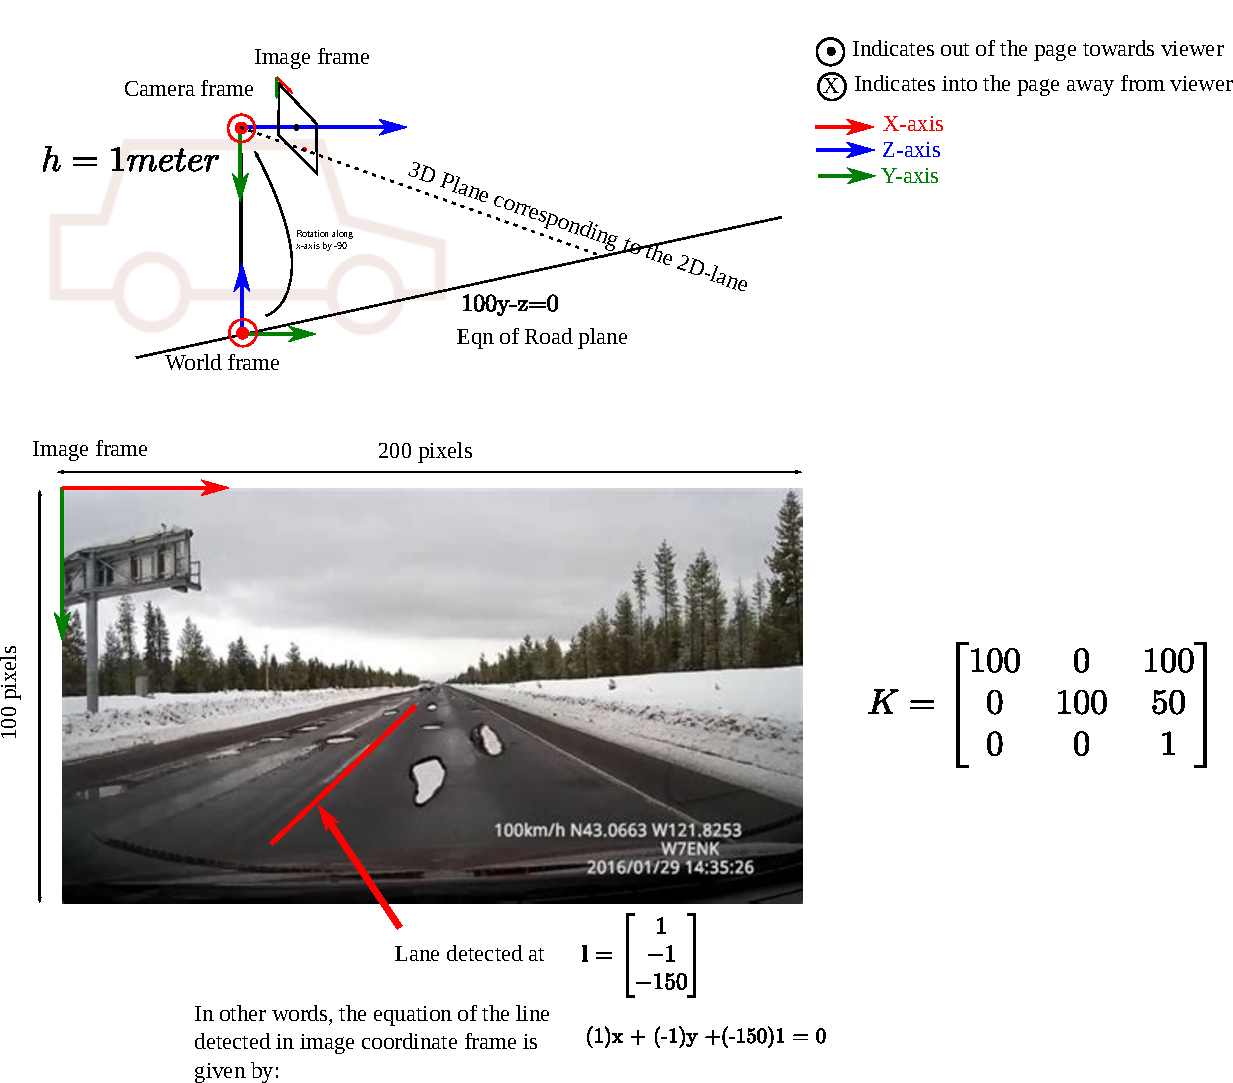
\includegraphics[width=\linewidth]{media/image-road-triangulation-line-plane.pdf}
  \caption{Line-plane triangulation}
  \label{fig:line-plane-triangulation}
\end{figure}

\newpage
.
\newpage

\begin{prob}
  Find the minimum point of the function, $f(\bfu) = 2 \bfu^\top A^\top A \bfu - 3 \bfu^\top\bfb +
  4 \bfc^\top \bfu + d$. Let $\bfu \in \bbR^{n \times 1}$ be a n-dimensional vector and sizes of $A, \bfb, \bfc, d$
  be such that matrix multiplication and addition is valid. Also assume that $A^\top A$  is
  full rank, hence invertible.
\end{prob}

\paragraph*{Solution}
Watch this lecture \url{https://drive.google.com/file/d/1wgY2LAw7LQnh_IyHY0XDAr2yorXta93Z/view?usp=sharing}

\begin{prob}
  Let matrix $A \in \bbR^{m \times n}$ be a $m \times n$ matrix. We are given
  that $B = A^\top A$ has $n$ orthonormal eigen vectors $\bfe_1, \dots \bfe_n$ with
  corresponding eigen values as $\lambda_1 \dots \lambda_n$ such that $B\bfe_i =
  \lambda_i \bfe_i$ for all $i \in \{1, \dots n\}$. Let the rank of
  matrix $A$ be $r$. Write the thin singular
  value decomposition of $A = U_{m \times r} \Sigma_{r \times r} V^\top_{n
    \times r}$  in terms of eigen values and
  eigen vectors of matrix $B = A^\top A$.
\end{prob}

\paragraph*{Solution}
Go through these \href{https://vikasdhiman.info/ECE417-Mobile-Robots/slides/03-07-linear-algebra_files/main.pdf.pdf}{slides}.
Watch this lecture \url{https://drive.google.com/file/d/13aO_XI7kykQNOs5RJ0fhqtL5fgEzVfkN/view?usp=sharing}

The matrix of right singular vectors of $A$ is same as the eigen vector matrix
of $B = A^\top A$.
\begin{align}
  V &= \begin{bmatrix} \bfe_1 \dots \bfe_r \end{bmatrix} \in \bbR^{n \times r}
\end{align}

The matrix of singular values are the square root of eigen values of $B$.
\begin{align}
  \Sigma &= \begin{bmatrix}
    \sqrt{\lambda_1} & \dots & 0 \\
    0 &  \ddots & 0 \\
    0 & \dots & \sqrt{\lambda_r} \\
    \end{bmatrix} \in bbR^{r \times r}
\end{align}

\begin{align}
  U &= \begin{bmatrix} \bfu_1 \dots \bfu_r \end{bmatrix} \in \bbR^{m \times r}
  \\
  \text{where } \bfu_i &= \frac{A\bfe_i}{\sqrt{\lambda_i}}
\end{align}
\newpage

\begin{prob}
  Let matrix $A \in \bbR^{m \times n}$ has the singular value decomposition
  (SVD) as $A = U\Sigma V^\top$ and rank of the matrix be $r = \text{rank}(A)$.
  Write the basis vectors of the four fundamental subspaces of matrix $A$ in
terms of SVD,
  \begin{enumerate}
    \item Null space of $A$ ($\calN(A) = ?$).
    \item Column space or range space ($\calR(A) = ?$).
    \item Row space ($\calR(A^\top) = ?$).
    \item Left null space ($\calN(A^\top) = ?$).
  \end{enumerate}
  You can denote the first $r$ column vectors of $U$ has $U_{1:r} \in \bbR^{m
    \times r}$ and the
  renaming $m-r$ vectors as $U_{r+1:m} \in \bbR^{m \times (m-r)}$. Similarly for
$V$, first $r$ column vectors of $V_{1:r} \in \bbR^{n \times r}$ and $V_{r+1:n}
\in \bbR^{n \times (n-r)}$.
\\
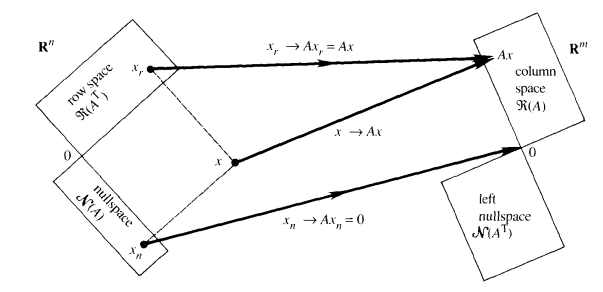
\includegraphics[width=0.7\linewidth]{media/four-fundamental-subspaces.png}
\end{prob}
\newpage
\paragraph*{Solution}
Watch lecture \url{https://drive.google.com/file/d/17Cr0rMr567gfRNrrj9ri9vtsFaNLqW7t/view?usp=sharing}

\begin{enumerate}
\item Null space of $A$ ($\calN(A) = V_{r+1:n}$).
\item Column space or range space ($\calR(A) = U_{1:r}$).
\item Row space ($\calR(A^\top) = V_{1:r}$).
\item Left null space ($\calN(A^\top) = U_{r+1:m}$).
\end{enumerate}

\section*{Extra practice problems}

\begin{prob}
  Find a line passing through the following points 
  \begin{align*}
    \bfu_1 = [101, 203]^\top,
    \bfu_2 = [49, 102]^\top,
    \bfu_3 = [27, 51]^\top,
    \bfu_4 = [201, 403]^\top,
    \bfu_5 = [74, 151]^\top.
    \end{align*}
    You can leave the output in terms of SVD.
\end{prob}

\begin{prob}
  Find a plane passing through the following points 
  \begin{align*}
    \bfx_1 = [9.99, 101, 203]^\top,
    \bfx_2 = [5.1, 49, 102]^\top,
    \bfx_3 = [2.5, 27, 51]^\top,
    \bfx_4 = [21, 201, 403]^\top,
    \bfx_5 = [7.6, 74, 151]^\top.
  \end{align*}
  You can leave the output in terms of SVD.
\end{prob}

\begin{prob}
  Find the 3D line in parameteric representation that is formed by the intersection of two planes $\bfp^\top \underline{\bfx} = 0$ (with $\bfp = [1, 2,
  3, 4]^\top$)  and $\bfq^\top \underline{\bfx} = 0$ where $\bfq = [-3, 2, 1, 4]^\top$.
\end{prob}

\begin{prob}
  Find the point on the intersection of following 3D lines $\bfx = \lambda_1
  \bfd_1 +  \bfy$ and $\bfx = \lambda_2 \bfd_2 + \bfz$. Here $\lambda_1\in \bbR$ and
  $\lambda_2 \in \bbR$ are the free parameters. The rest of the parameters have
  the following values
  \begin{align*}
    \bfd_1 = [1, 2, 0]^\top,
    \bfd_2 = [-2, 1, 0]^\top,
    \bfy = [1, 2, 0]^\top,
    \bfz = [4, 5, 0]^\top
    \end{align*}
\end{prob}

\begin{prob}
  Find the point of intersection of the 3D line $\bfx = \lambda \bfd + \bfx_0$ with
  the 3D plane $\bfp^\top \underline{\bfx} = 0$. The parameters have the
  following
  \begin{align*}
    \bfd = [1, 2, 0]^\top, \bfx_0 = [3, 4, 5]^\top, \bfp = [1, 2, 0, 7]^\top
  \end{align*}
\end{prob}

\newpage
\section*{Practice problem solutions}
\paragraph*{Solution 6}
Watch lecture \url{https://drive.google.com/file/d/13aO_XI7kykQNOs5RJ0fhqtL5fgEzVfkN/view?usp=sharing}
Let $\bfl \in \bbP^2$  be the parameters of the line, so that $\ubfu^\top \bfl = 0$.
\begin{align*}
  A = \begin{bmatrix}
    \bfu_1^\top & 1 \\
    \bfu_2^\top & 1\\
    \bfu_3^\top & 1\\
    \bfu_4^\top & 1\\
    \bfu_5^\top & 1
    \end{bmatrix}_{5 \times 3}
\end{align*}
We are looking for the solution of $A \bfl = 0$.
Let the SVD of $A = U\Sigma V^\top$. Let $V = [\bfv_1, \bfv_2, \bfv_3]$, then
the representation of the line $\bfl = \bfv_3$.

\paragraph*{Solution 7}

Watch the lecture \url{https://drive.google.com/file/d/1PEdgHCf6Ud0WYMVtCRlsjfctDcnBm8E9/view?usp=sharing}

Let $\bfp \in \bbP^3$  be the parameters of the plane, so that $\underline{\bfx}^\top \bfp = 0$.
\begin{align*}
  A = \begin{bmatrix}
    \bfx_1^\top & 1 \\
    \bfx_2^\top & 1\\
    \bfx_3^\top & 1\\
    \bfx_4^\top & 1\\
    \bfx_5^\top & 1
  \end{bmatrix}_{5 \times 4}
\end{align*}
We are looking for the solution of $A \bfp = 0$.
Let the SVD of $A = U\Sigma V^\top$. Let $V = [\bfv_1, \bfv_2, \bfv_3, \bfv_4]$, then
the representation of the line $\bfp = \bfv_4$.
\paragraph*{Solution 8}
Watch the lecture \url{https://drive.google.com/file/d/1JaEwLxQ2BvT30sVxshmglBz_v5FjC1hW/view?usp=sharing}
$\bfx = \lambda (\bfp_{1:3} \times \bfq_{1:3}) + \begin{bmatrix} \bfp_{1:3}^\top
  \\ \bfq_{1:3}\end{bmatrix}^\dagger \begin{bmatrix}-p_4 \\ q_4 \end{bmatrix}$
\paragraph*{Solution 9}
Watch the lecture \url{https://drive.google.com/file/d/1foVVQBC0krljjJ3f-UP4zsHn4l-c611e/view?usp=sharing}
\[
  \begin{bmatrix}\bfd_1& -\bfd_2\end{bmatrix}\begin{bmatrix} \lambda_1 \\
    \lambda_2\end{bmatrix} = \bfz - \bfy
  \]
  or
  \[ \begin{bmatrix} \lambda_1 \\
      \lambda_2\end{bmatrix} = \begin{bmatrix}\bfd_1&
      -\bfd_2\end{bmatrix}^\dagger \bfz - \bfy
    \]
    The point of intersection is given by
    \[ \bfx = \lambda_1 \bfd_1 + \bfy \]
\paragraph*{Solution 10}

Watch the lecture \url{https://drive.google.com/file/d/1wgY2LAw7LQnh_IyHY0XDAr2yorXta93Z/view?usp=sharing}
\[
  \lambda \bfp_{1:3}^\top \bfd + \bfp_{1:3}^\top \bfx_0  + p_4 = 0
  \]
  Solve for $\lambda$.
  \[
    \lambda = -\frac{\bfp_{1:3}^\top \bfx_0  + p_4}{\bfp_{1:3}^\top \bfd}
    \]
    Point of intersection is
    \[
      \bfx = \lambda \bfd + \bfx_0
      \]


\end{document}
